\section{Semiconductor Detectors}
\subsection{General Remarks}
\begin{figure}[ht]
    \centering
    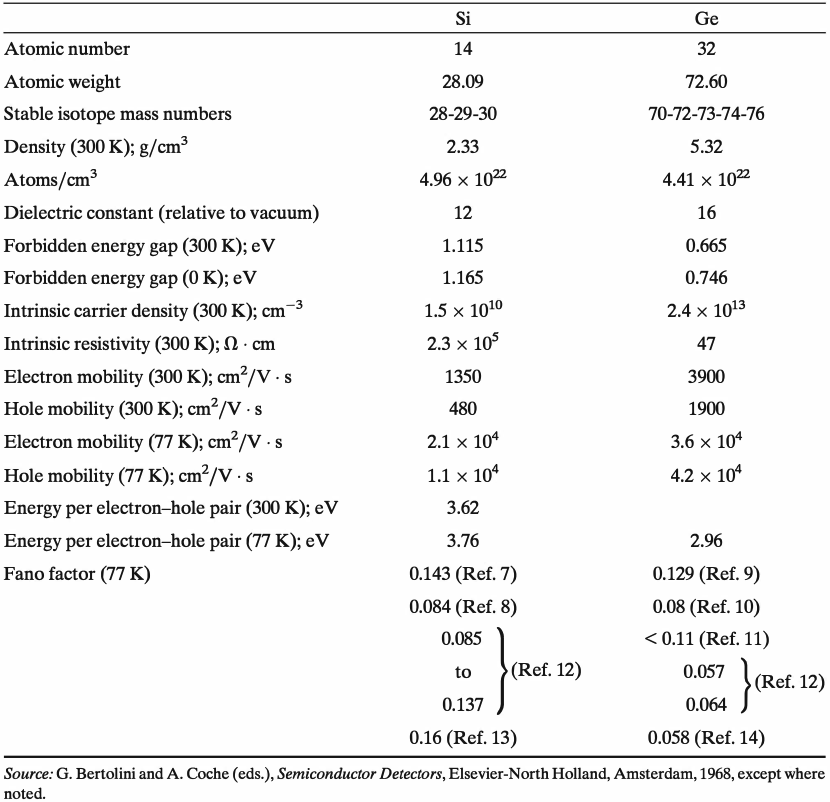
\includegraphics[width=1.0\textwidth]{images/Si_Ge_properties.png}
    \caption{Intrinsic properties of Si and Ge.}
    \label{fig:Si_Ge_properties}
\end{figure}
\subsubsection{Advantages or Semiconductor Detectors}
\begin{itemize}
    \item Good energy resolution due to small energy to generate information carriers (electron-hole pairs)
    \item High-density (solid)
    \item Good charge carrier collection properties
    \item Good timing characteristics
\end{itemize}
\subsubsection{Semiconductor vs. Gas Detectors}
\begin{itemize}
    \item Similarities:
    \begin{itemize}
        \item Ionization of detector material creating positive and negative charge carriers 
        \item Drift and collection of charge carriers due to external electric field
        \item Induction of signal during charge collection due to motion of charge carriers
    \end{itemize}
    \item Differences:\\
    A semiconductor detectors has
    \begin{itemize}
        \item Solid state counter with higher density and ($dE/dx$)
        \item Smaller energy to generate charge carriers
        \item Higher mobility
        \item Both types of charge carriers are fast
    \end{itemize}
\end{itemize}
\subsection{Principles of Operation}
\subsubsection{Band Gap and Ionization Energy}
\begin{figure}[ht]
    \centering
    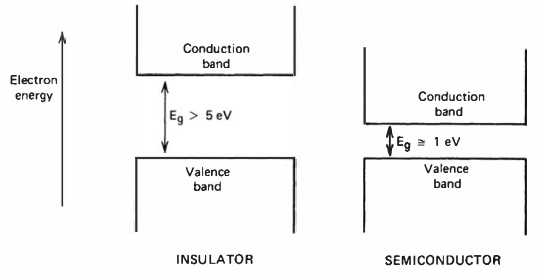
\includegraphics[width=0.5\textwidth]{images/semiconductor_band_structure.png}
    \caption{Band structure for insulators and semiconductors.}
    \label{fig:semiconductor_band_structure}
\end{figure}
\begin{itemize}
    \item In band theory, the energy of any electron within the pure material is confined to allowed energy bands, which may be separated by gaps or ranges of forbidden energies. As shown in figure~\ref{fig:semiconductor_band_structure}, the valence band corresponds to outer-shell electrons that are bound to specific lattice sites within the crystal; the conduction band represents electrons that migrate freely through the crystal. The band gap separates the two bands.
    \item Excitations in the crystal, where a valence electron gains sufficient energy to be elevated across the band gap into the conduction band, creates an electron-hole pair, analogous to a ion pair in gases. Ionizing radiation creates electron-hole pairs in the semiconductor as charge and information carriers. 
    \item As shown in the table below, the ratio of W to band gap is approximately constant for a wide range of materials, reflecting the constant ratio between electron-hole generation and phonon generation. See figure~\ref{fig:Si_Ge_properties} for more detailed Si and Ge intrinsic properties.
    \begin{center}
        \begin{tabular}{|c|c|c|c|}
        \hline
         &  Mean Ionization Energy W (eV) & Density (g/cm$^3$) & Fano Factor \\
        \hline
        Gases     & 30 & $7\sim50\times10^{-4}$ & $0.1\sim0.2$ (ionization vs. excitation)\\
        \hline
        Si & 3.62 & 2.33 & $\sim0.10$ (ionization vs. phonons)\\
        \hline
        Ge & 2.96 & 5.32 & $\sim0.10$ (ionization vs. phonons)\\
        \hline
        \end{tabular}
    \end{center}
\end{itemize}
\subsubsection{Lattice, Intrinsic Carrier Density,  Mobility, and Resistivity}
\begin{itemize}
    \item Lattice:\\
    Both Ge and Si have the diamond cubic crystal structure.
    \item Intrinsic carrier density:\\
    The intrinsic (no dopant) carrier density in a semiconductor is low.
    \begin{itemize}
        \item[] Assuming equilibrium between thermal excitation and recombination, 
        \item[] the concentration of electrons (or holes) $n_i=\sqrt{N_CN_V}\exp(-E_{Gap}/2k_BT)$
        \item[] , where $N_V$ and $N_C$ are the densities of states in the valence and conduction bands.
        \item[] Typical values of $n_i$ are $2.5\times10^{13}$ cm$^{-3}$ for Ge and $1.4\times10^{10}$ cm$^{-3}$ for Si.
        \item[] However, for example in Si, the atomic density $n_{atoms}=\frac{N_A\rho}{M}\approx5\times10^{22}\;\text{cm}^{-3}$
        \item[] Therefore, $f=(1.5\times10^{10})/(5\times10^{22})=3\times10^{-13}$ 
    \end{itemize}
    \item Mobility ($\mu$) and resistivity ($\rho$):
    \begin{itemize}
        \item[] The drift velocity is given by $v_{e/h}=\mu_{e/h}E$
        \item[] Current density $J=\text{charge density}\times v=en_i(\mu_e+\mu_h)E$
        \item[] Since $J=\sigma E$ where $\sigma$ is conductivity,
        \item[] $\rho=1/\sigma=[en_i(\mu_e+\mu_h)]^{-1}$
        \item[] Assuming only thermal excitations, where $n_i=n_p=n_e$, 
        \item[] with $n_i=10^{10}\;cm^{-3}$ and $\mu_e=1500\;cm^2/Vs$, then $\rho\sim10^5\;\Omega\cdot cm$
    \end{itemize}
\end{itemize}
\subsubsection{Doped Semiconductors}
\begin{itemize}
    \item n-type:\\
    Doped with group V elements (donors), the current is mainly due to excess electrons
    \item p-type:\\
    Doped with group III elements (acceptors), the current is mainly due to excess holes
    \item p-n junction:\\
    A depleted (charge carrier free) zone can be created by combining n and p regions to form a p-n junction due to charge carrier diffusion. The electric field or contact potential caused by the new space charges stop the diffusion. See figure~\ref{fig:pn_junction_formation} for visualization of the process.
    \begin{figure}[ht]
        \centering
        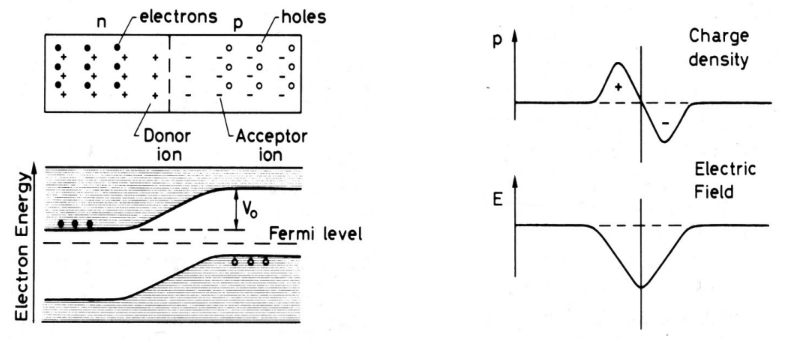
\includegraphics[width=0.5\textwidth]{images/pn_junction_formation.png}
        \caption{p-n junction formed due to charge carrier diffusion.}
        \label{fig:pn_junction_formation}
    \end{figure}
    \item Reverse-biased diode:\\
    By applying reverse bias, the depleted region of the p-n junction increases. See figure~\ref{fig:reverse_bias_diode}. 
    \begin{figure}[ht]
        \centering
        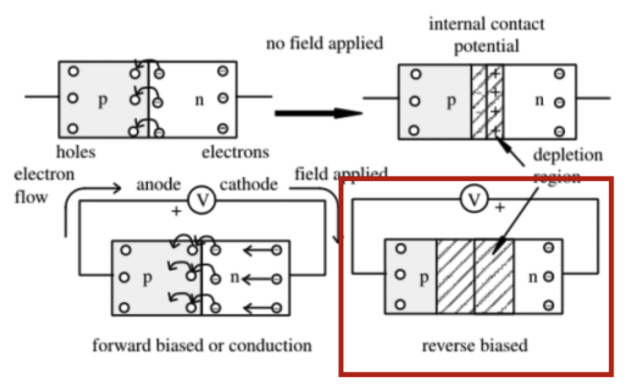
\includegraphics[width=0.5\textwidth]{images/reverse_bias_diode.png}
        \caption{Reverse-biasing of a diode.}
        \label{fig:reverse_bias_diode}
    \end{figure}
\end{itemize}
\subsubsection{Depletion Layer}

\subsection{Si Detectors}
\subsubsection{Varieties of Si Detectors}
\subsubsection{Si(Li) Detectors}
\subsubsection{Si Detector Applications}

\subsection{Ge Detectors}
\subsubsection{Overview}
\subsubsection{Planar and Coaxial Configurations}
\subsubsection{Energy Spectra and Efficiency}
\subsubsection{Varieties of Ge Detectors}

\subsection{Alternative Semiconductor Detectors}
\subsubsection{Limitations of Ge Detector Operations}
\subsubsection{Lifetime and Mobility}
\subsubsection{Charge Collection Properties}